\chapter{Introduction}
\markright{Huijuan Shao \hfill Chapter 1. Introduction \hfill}

\emph{Analytics} has transformed the perception of the world we live in. Big Data is the lingua franca of the twenty first century and data science has become an essential lens through which decision making is seen. The massive amounts of data collected via several active and passive instrumentations positions us truly in \emph{age of information}. Data via Web 2.0, social media, internet of things, traffic flow, gene sequencing, etc. in conjunction with advancement of data mining & machine learning to glean actionable insights has influenced the world in designing policy, pricing products, launching political campaigns, and many other applications. The power of \emph{data analytics}, thus, is in its diversity. 

One such application is in \emph{urban computing}, primarily from the perspective of data science. It has been projected that by the year 2030, cities will grow by 590,000 square miles and add an additional 1.47 billion people, so that 6 out of every 10 people will live in a city. Key issues concerning urban populations, such as public health, sustainable use of limited energy resources, emergency preparedness, and societal stability will rise to the forefront. Epidemiological analysis of public health data to analyze infection spread, traffic flow analysis via public transport and taxi cab data, election forecasting and e-governance, and the like are just few of the many examples of how dissecting the data can provide awareness and knowledge about the society we live in. A data scientist role has become critical in being able to learn, process, analyze, and deliver actionable insights that can help realize the promises of this \emph{unprecedented urbanization}. 

Towards that end, one of the critical components which has long been a topic of research interest but has found resurgence in this era of urbanization is tackling problems of energy consumption. Sustainable energy supply to cities is more critical now than ever before. Moreover, the relevance of the problem is two-fold. The immediate impact of urbanization has presented us with logistical problems. How do we meet the needs of the rapidly growing cities? Can we design \emph{smart buildings} and \emph{smart neighborhoods} that optimizes energy consumption? Answering these questions is critical to the economy of the country and the economy of the society at large. The larger impact is one that energy industry has on the environment. While renewable energy sources are being investigated, fossil fuels remain the prime source of energy supply. Climate-change is a huge problem that will have an impact on humanity as we know it. It is a problem that needs a several pronged attack to find a solution and finding solutions to problems in energy consumption, reducing the carbon footprint, would be a big step forward.

One of the essential resources in today's world is power and electricity. Needless to say, electricity usage permeates all aspects of modern society.
Its most conspicuous
uses include urban contexts such as
lighting, air conditioning, refrigeration, heating, and, powering
appliances and gadgets but its penetration is pervasive across rural
and industrial sectors.
In 2014, the residential and commercial sector
comprised nearly 40\% of all the electricity generated in the U.S. \cite{book2014us}.
Furthermore, our dependence on electricity will continue to grow
as emphasis shifts away from fossil fuel based vehicles to electric
vehicles.

 

While people generally agree on the importance of conservation and
usage curtailment, they are often at difficulties to quantify 
{\em where, when} and {\em how much} electricity is consumed.
Typically, residences and businesses receive
monthly electricity bills indicating aggregate usage, with no information on
the breakdown of consumption by appliances/devices, time of day, or day of
week (this is an area in great flux, however). Research has 
shown that simply making such feedback available to users
can reduce consumption by up to 50\%, although typical saving 
are in the 9\% to 20\% range \cite{book2014us}.%\cite{energydatabook2011}.

One obvious approach to determining the breakdown of consumption is to install
power meters in every circuit (and sub-circuit)
to capture consumption of individual devices in homes and
offices. Such installation is costly and intrusive, making 
this option unviable in practice. 
An alternate
solution, called energy disaggregation or non-intrusive load monitoring
(NILM),
first proposed by Hart~\cite{hart1992}, is to use analytics to 
{\em infer} the breakdown of consumption from an aggregate 
power measurement of a
site. This drastically reduces the number of meters required per 
home/installation, typically to just one. Furthermore, depending on the analytics desired, it is possible to
use the measurements already being recorded by a utility meter for
disaggregation, especially in cases where utility companies have deployed
smart meters.
Energy disaggregation is hence today a booming area offering both
challenging problems for data analytics and having practical relevance in a
number of areas including sensor networks and building analytics.

Another approach to save energy in homes is to 
efficiently use electricity devices.  
In residential buildings, 
the biggest consumer of electricity is usually the HVAC 
(heating, ventilation, and cooling) system, which generally accounts for ~54\% 
of the buildings electricity consumption~\cite{book2014us}. 
How to automatically start up and shut down the HVAC unit 
is thus a key problem. 
One solution is to predict the occupancy at home 
is to begin by analyzing the activities of daily life 
inside the building. 
Based on the occupancy information, 
an automatic control system can be installed
to operate the HVAC. 

In this work we make efforts to resolve some of the problems arising in smart building research with 
temporal mining approaches.
\begin{enumerate}
	\item We present a survey on energy disaggregation from the perspective of data mining features and supervised, semi-supervised and unsupervised algorithms. 
	\item The temporal mining approach motif mining works effectively for energy disaggregation. 
	\item We utilize multivariate piecewise motif mining algorithm for both energy disaggregation and water disaggregation. 
	\item The episode-based model Episode Generating HMM (EGH) and a mixture of EGHs performs well for event prediction in occupancy prediction. 
	%\item It can be used for supervised learning disaggregation and semi-supervised learning approach, even for un-supervised learning approach. 
\end{enumerate}
\section{State of the art}
We open the thesis by defining energy disaggregation formally. Briefly, the goal of energy disaggregation is to effectively break down appliance level power consumption. We conduct a complete survey of several mechanisms and techniques that employ data mining and machine learning to tackle energy disaggregation. While surveys have been conducted in the past, most of them are presented from an electrical engineering perspective. We survey works that use supervised and unsupervised learning. We compare and contrast a range of algorithms that have been used for energy disaggregation. Our self-contained survey introduces the necessary electrical engineering concepts that are required for data scientists to conduct research in the space, describe necessary tools and datasets to develop and test algorithms. We describe how experimental testbeds should be setup and how to record data from the necessary sensors and meters. Moreover, we also present some promising directions of research in the space from a data mining perspective. Essentially, we provide a \emph{one-stop-shop} starting point for data mining practitioners to understand the problem scope of energy disaggregation, expose themselves to the problems, and then conduct research in the space.

\section{Temporal Mining}
One of the important forms of data is based on time. Temporal data mining revolves around the techniques (algorithms) that enumerate structures, patterns, and signatures over temporal data (time series, for instance). In this thesis we focus on three temporal mining algorithms. 

\subsection{Motif Mining}
Motif mining was a temporal data mining technique that was initially proposed in the \textbf{put motif mining cites} and it was extensively studied in \textbf{please put second motif mining cites}. Basically the fundamental idea behind \emph{motif mining} is that it symbolically encodes the numerical time series data. After which, the symbols combine to form episodes in the data resulting in patterns that can be mined. Furthermore by combining domain specific information and pattern mining techniques, we extract frequent meaningful episodes from the symbolized time series.

Furthermore when there are multiple time series that describe the data, we employ \emph{multi-variate motif mining} to find meaningful patterns. The algorithms for multi-variate temporal motif mining are similar to the univariate case, except that the symbolic encoding is represented as a vector. Therefore each time point in the data is represented as a vector of symbols, with each symbol corresponding to one of the several time series that represents the data. Now, the combination of these vector symbols forms episodes that can be mined from the multi-variate time series data. Again by combining domain specific knowledge, we extract meaningful episodes from the data.



\subsection{Episode Generating Hidden Markov Model (EGH)} A hidden markov model is an ubiquitous construct to model time series data. It is a tool for representing probability distributions over a sequence of data. The hidden Markov model gets its name from two important properties. The observation (data point) was generated by some process whose state is \emph{hidden} from the observer. Second, the state of this hidden process satisfies the \emph{Markov} property that the current state is independent of all prior states. The \emph{Episode Generating HMM}, researched in \textbf{put cites of EGH, please} connects the episodes with an HMM model and it has a parameter to evaluate whether an episode is frequent or not. A mixture of EGH describes a situation that several frequent episodes are embedded into a time series. It can be used to predict whether a target symbol will be the next symbol in a time series.



\section{Applications of Motif Mining and EGH}
In our work we apply motif mining techniques, both univariate and multivariate cases, to energy disaggregation. By correlating episodic information with the switching on and off of appliances from time-series represented energy data we are able to successfully determine the one-one mapping between a certain appliance and it's usage patterns and time. Our results are presented in Chapter 4.

The formulation of the EGH model lends itself to predicting occupancy in a residence or any building. We develop an EGH model based for occupancy prediction that can assist in automated turning on or off of the HVAC system, which can single-handedly reduce a good portion of the energy consumption footprint. We demonstrate that our algorithm can effectively forecast occupancy.  We present our analysis in Chapter 5.

The rest of the thesis is organized as follows. Chapter 3 presents a survey on energy disaggregation. Chapter 4 describes our solution to energy disaggregation and Chapter 5 discusses our solution to the occupancy prediction problem. We conclude the thesis in Chapter 6 with some discussion and future directions of research.  

%A related problem pertains to
%non-invasive indoor activities tracking.
%The goal here is to predict the locations of people inside a building
%without the use of invasive cameras.

%\section{Timeline}
%The first proposed
%research problem
%on energy disaggregation has been completed although 
%the work will be extended to time-based motif mining and 
%a new probabilistic models.
%The second task of activity of daily life patterns is underway. 
%The third subject on non-invasive indoor activities tracking 
%will start in this Oct.. 
%A timeline of activities is shown in Figure~\ref{fig_PhDtimeline}. 

%\begin{figure}[!hbtp]
%\centering
%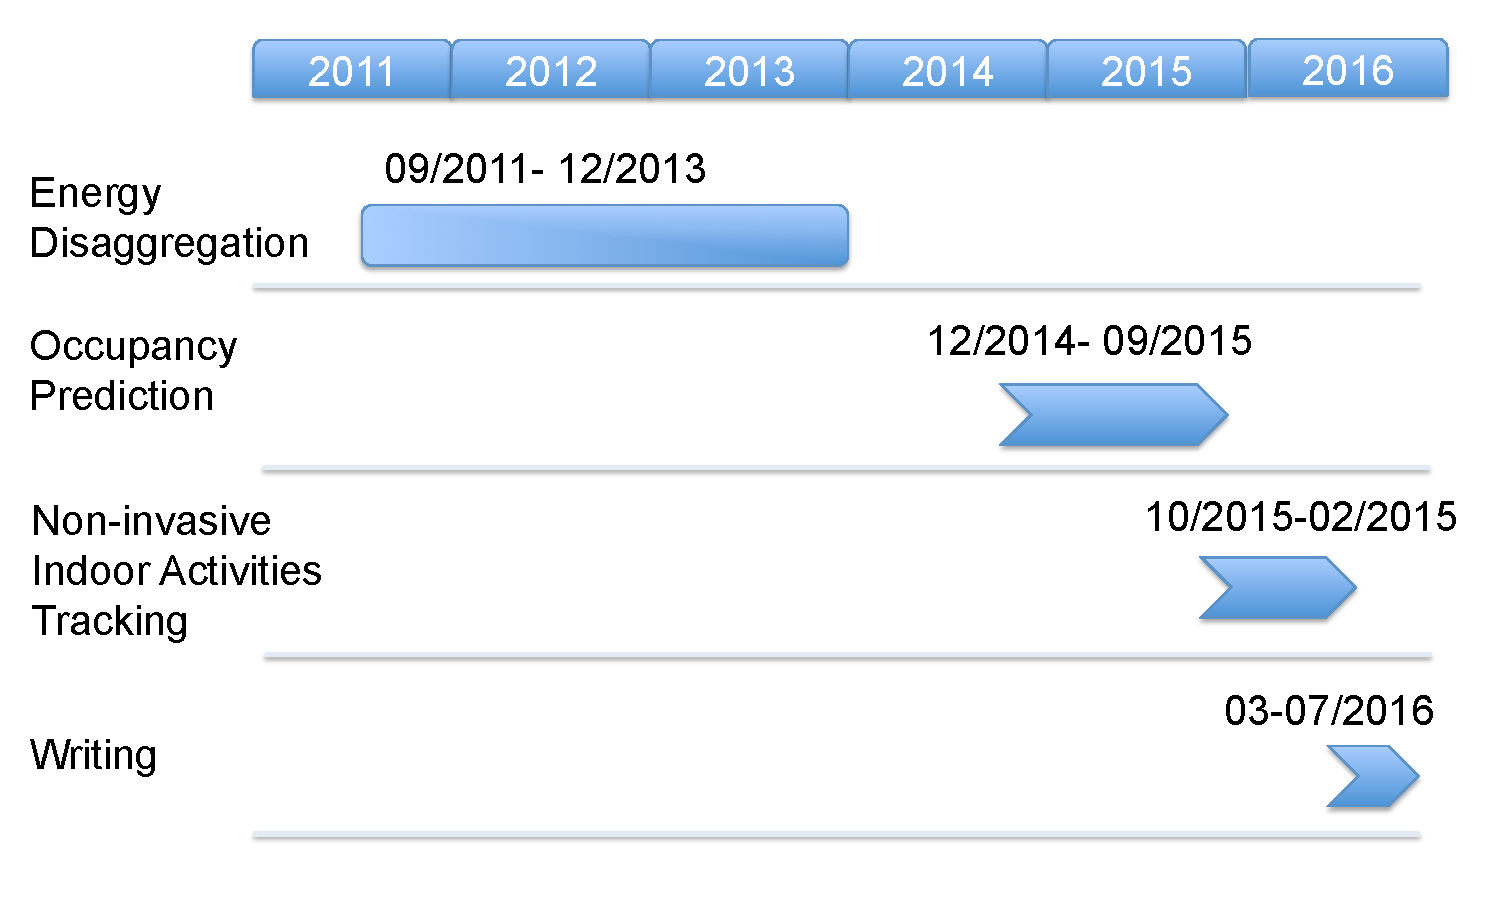
\includegraphics[width=0.8\textwidth]{fig/PhDTimeline.pdf}
%\caption{Timeline.\label{fig_PhDtimeline}}
%x\end{figure}
